\documentclass{beamer}
\usetheme{CambridgeUS}
\title[Process]{The Koopman operator identification algorithm}
\subtitle{So far}
\institute[Polimi]{Politecnico di Milano}
\author{Sergio Vanegas}
\date{\today}

\usepackage{listings}
\usepackage[framed,numbered,autolinebreaks,useliterate]{mcode/mcode}

\usepackage{xcolor}

\usepackage{siunitx}

\usepackage{caption}
\usepackage{subcaption}

\begin{document}

\begin{frame}[plain,noframenumbering]
    \maketitle
\end{frame}

\begin{frame}{Table of Contents}
    \tableofcontents
\end{frame}


\section{Robust Koopman}

\begin{frame}{Frobenius regularization - Formulation}
    We start by following the proposed reformulation of the minimization problem proposed in \textit{Robust tube-based model predictive control with Koopman operators} as follows:

    \begin{equation*}
        \overline{\mathcal{K}}_N =
        \min_{\mathcal{K} \in \mathbb{R}^{\tilde{N} \times N}}
        \sum_{k=1}^K \left[
            \left|\left|
                \mathbf{g}\left(\mathbf{y}\left[k\right]\right) - 
                \mathcal{K}
                \begin{pmatrix}
                \mathbf{g}\left(\mathbf{x}\left[k\right]\right)
                \\
                \mathbf{u}\left[k\right]
                \end{pmatrix}
            \right|\right|^2
            {
                \color{red}
                + \alpha\left|\left|\mathcal{K}\right|\right|_F^2
            }
        \right],
    \end{equation*}

    where

    \begin{itemize}
        \item $\mathbf{g}$ is the observable vector,
        \item $K$ is the total number of snapshots,
        \item $\left(\mathbf{x},\mathbf{y}\right)$ are the snapshot pairs,
        \item $\mathbf{u}$ is the input vector,
        \item $\left|\left|\cdot\right|\right|_F$ is the element-wise 2-norm (Frobenius norm).
    \end{itemize}
\end{frame}

\begin{frame}[fragile]{Frobenius regularization - MATLAB implementation}
    \begin{lstlisting}[language=Matlab,basicstyle=\tiny]
function [A,B] = Koopman(X,Y,U,alpha)
    options = optimoptions(@fminunc, ...
                        'Display', 'final', ...
                        'UseParallel', true, ...
                        'OptimalityTolerance', 1e-3, ... % Default is 1e-6
                        'StepTolerance', 1e-3, ...
                        'MaxIterations', 250); % Default is 400
    for i=1:size(Y,1)
        m0 = V(i,:)/G;

        if alpha>0.0
            fun = @(m) sum((Y(i,:)-m*[X;U]).^2) ...
                    + alpha*sum(m.^2);

            % No longer LSqr, since the Frobenius norm is considered separately
            m = fminunc(fun,m0,options);
        elseif alpha==0.0
            m = m0;
        end

        A(i,:) = m(1:size(X,1));
        B(i,:) = m(size(X,1)+1:end);
    end
end
    \end{lstlisting}
\end{frame}


\section{From prototyping to implementation}

\begin{frame}{Language alternatives - Benchmark formulation}
    Considering the performance limitations of a high-level interpreted languages, some alternatives had to be considered. The evaluated candidates were:

    \begin{itemize}
        \item Python: still high-level, but further optimized because of its open-source nature. Development complexity equivalent to that of MATLAB.
        \item C++: compiled language, and a classical choice for scientific programming. Even if complex, the development process is facilitated by the broad library collection available.
        \item Rust: memory-safe compiled language that pretends to replace C/C++ in the following years. High development complexity given it's in its early stages.
    \end{itemize}

    A simple benchmark based on the performance of ODE data generation (which evaluates both matrix and nonlinear implementations) was set up.
\end{frame}

\begin{frame}{Language alternatives - Benchmark results}

    \begin{itemize}
        \item MATLAB

        \begin{itemize}
            \item User time: $\SI{26.05}{\second}$
            \item Wall clock time: $\SI{28.62}{\second}$
            \item Maximum resident set size: $782348$ kb
        \end{itemize}

        \item Python

        \begin{itemize}
            \item User time: $\SI{25.44}{\second}$
            \item Wall clock time: $\SI{26.21}{\second}$
            \item Maximum resident set size: $59880$ kb
        \end{itemize}

        \item C++
        
        \begin{itemize}
            \item User time: $\SI{0.70}{\second}$
            \item Wall clock time: $\SI{1.76}{\second}$
            \item Maximum resident set size: $4320$ kb
        \end{itemize}

        \item Rust
        
        \begin{itemize}
            \item User time: $\SI{0.54}{\second}$
            \item Wall clock time: $\SI{6.44}{\second}$
            \item Maximum resident set size: $2736$ kb
        \end{itemize}
    \end{itemize}
    
\end{frame}

\begin{frame}{Language alternatives - Accuracy verification}
    \begin{figure}
        \centering
        \begin{subfigure}[b]{0.3\textwidth}
            \centering
            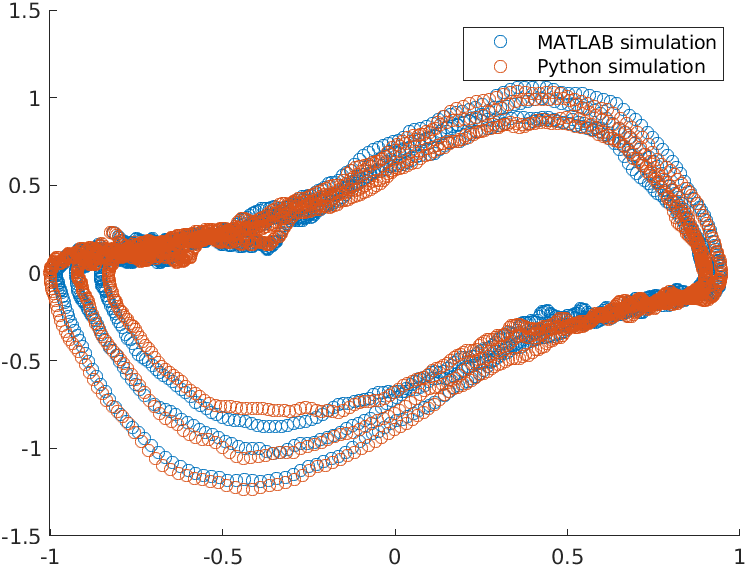
\includegraphics[width=\textwidth]{Python_Sim.png}
            \caption{Python - Simulated trajectory}
            \label{fig:sim_python}
        \end{subfigure}
        \hfill
        \begin{subfigure}[b]{0.3\textwidth}
            \centering
            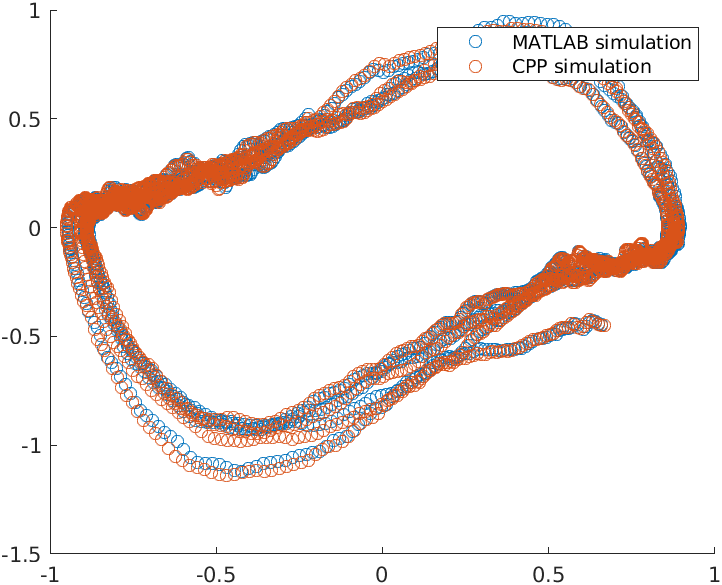
\includegraphics[width=\textwidth]{Cpp_Sim.png}
            \caption{C++ - Simulated trajectory}
            \label{fig:sim_cpp}
        \end{subfigure}
        \hfill
        \begin{subfigure}[b]{0.3\textwidth}
            \centering
            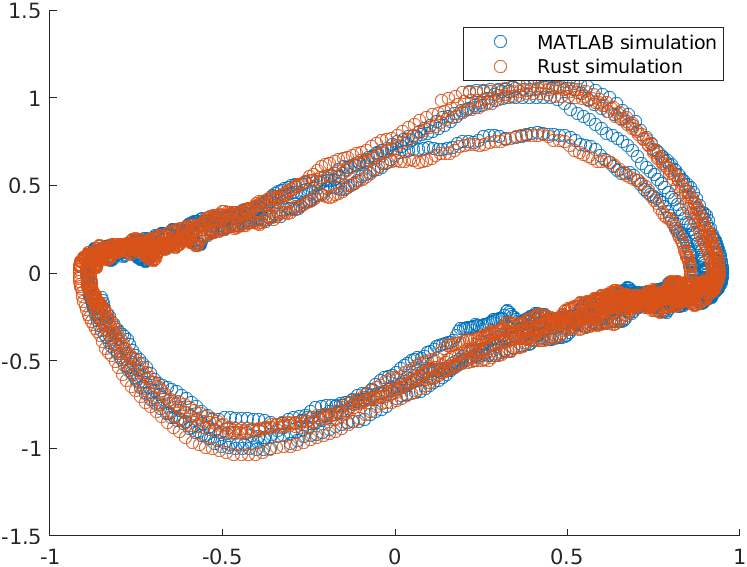
\includegraphics[width=\textwidth]{Rust_Sim.png}
            \caption{Rust - Simulated trajectory}
            \label{fig:sim_rust}
        \end{subfigure}
        \caption{Simulated trajectories (MATLAB simulation as reference)}
        \label{fig:implementations}
    \end{figure}
\end{frame}

\end{document}